\documentclass{csfourzero}

\title{CS4040 Report Structure}
\author{Timothy J.\ Norman}
\date{\today}
% A useful package to support on-line references
\usepackage{url}
\usepackage{natbib}

\bibliographystyle{plain}
\abstract{An expansion of the title and a contraction of the report. "this report invesigates", "similar pieces of work / related work is discussed", "results showed, it was found OR a "relevent con is given (dont need the overall result)""}


\begin{document}
\maketitle

\section{Introduction}
\label{sec:intro}

The aim of the introduction is to say what you are going to investigate in the report and why it
  is interesting.

Guide length: 250 words.

"The research interest of the paper", "evaluate the difference", explain the problem, define terms, why interesting / useful, "this report is organised as follows, list sections"

reference any formalisms and define the terms you use (or reference), short overview of what's to be investigated and why this is of interest, report is organised as follows...




\section{Background and related work}
\label{sec:lit}

A review of related work \cite{p2pbookv2,Burnett,p2pwiki}.

Guide length: 500 words.

further explain terms and problem and reading you have done - even if not papers, give a focus for my paper, "others have looked into...", only need 2-3 relevant papers that are well discussed.

Ok to say there has been limited work on a topic, have a got at explaining why.

\section{Research question}
\label{sec:rq}

Given the problem context (Section~\ref{sec:intro}) and background
(Section~\ref{sec:lit}), you should now be in a position to present
what you have investigated. \textbf{Pose this as a question.}

Then you should present your approach to addressing this
question.

Guide length: 500 words.

"intro why asking questions", "the questions are as follows", "At which point does", and as a second "is there a significant difference between the search engines"

"in order to answer this", "overview", explanation of tools

"the datasets...", explain how generated, how controlled, list all the variables in the data (suggested in the design section)

How the results are recorded and on what they will be compared (precision recall), or use accuracy? Need to explain why, accuracy might be appropriate for my experiment. This is a summary of the following section. High level parameters for the tools and generally how the subject are compared.

\section{Experimental Design}
\label{sec:exp}

What are your hypotheses? How are you going to test them? What is your
target population? What are your datasets; i.e.\ your sample of the
target population. What are the dependent and independent variables?

Guide length: 500 words.

first state the null hyps, one per question it seems, "significantly different" is the phrase to use it seems. can also state the alternatives if they are not clear.

detail test data and give justification for decisions

"To test these hyps [what happens in the experiement]", "this was then repeated for each..."

talk about the datasets that will be used. talk about the variables ()

\section{Results}
\label{sec:results}

Present the results. A good way to organise this is via subsections
for each hypothesis you tested. Include graphs of results
(e.g.\ Figure~\ref{fig:data}), tests of significance, etc. If you have
negative results, include them. A negative results is just as
informative and useful as a positive one, sometimes more so.

\begin{figure}
\centerline{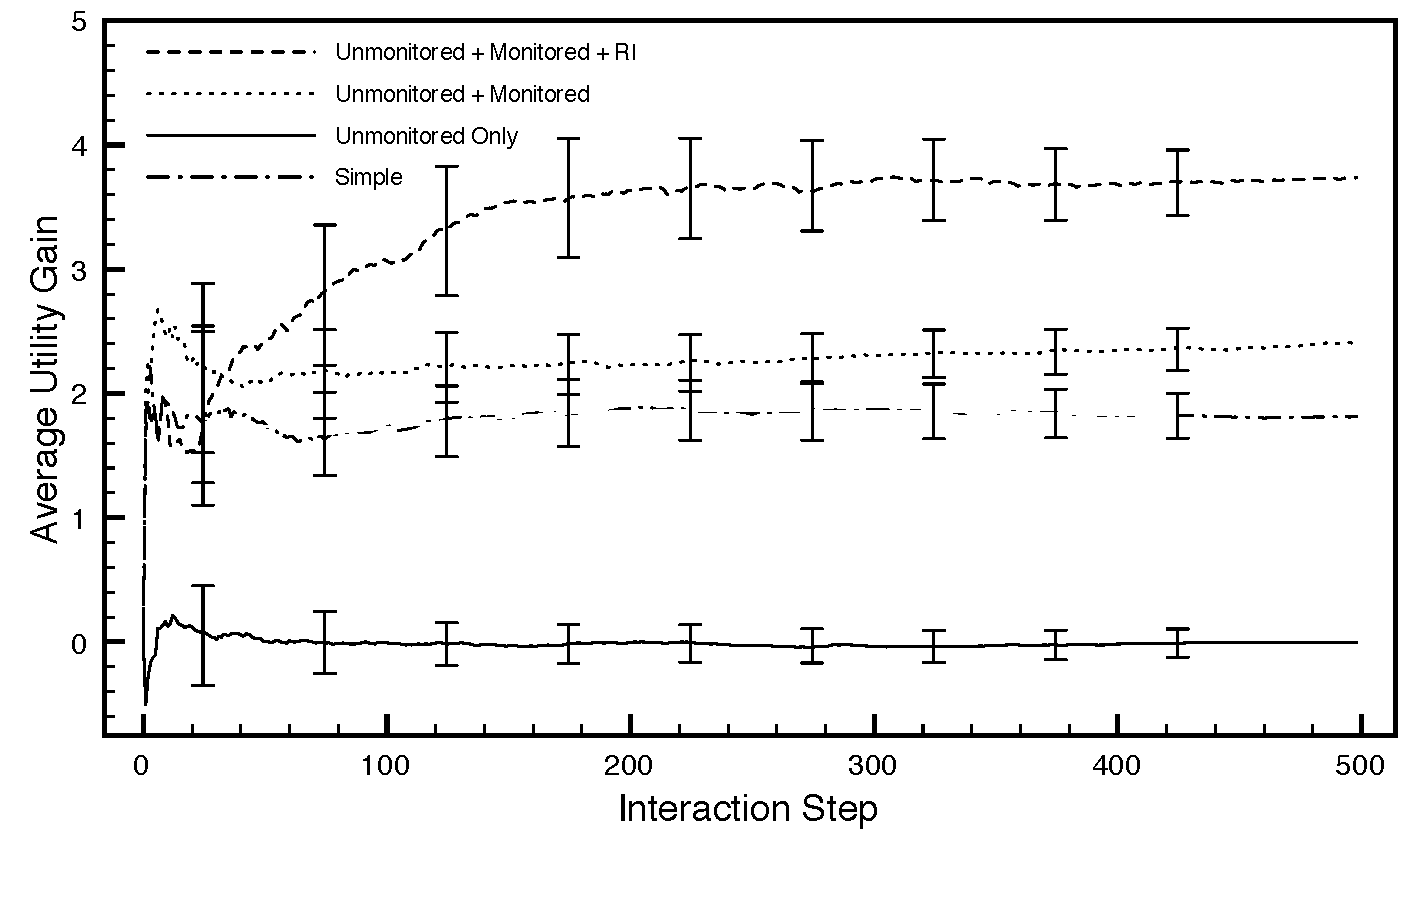
\includegraphics[width=5in]{basic-data-errors}}
\caption{Some results.}\label{fig:data}
\end{figure}

Guide length: 500 words.

table of the results in summary, same sentence ref a graph of the table.

the results suggest that all decreased in accuracy as the number of corruptions increased. Also x did better then y - quote values to support / highlight things in the table

then do a section for each comparison and hypothesis / quesion 5.1 5.2 - say was was and was not significant, in response to the question. Quote those p values!

Segment the section based on the number of questions, accuracy vs speed etc. for each quote the values of the statistical tests.

\section{Discussion}
\label{sec:discuss}

What do the results say? What have you learned from the
experiments? Have you identified a correlation between variables, or
causation? What are the limitations of what you've done? What further
experiments might be of benefit?

Guide length: 400 words.

results summary, state the relationships at a high level, make references to the values of the tests mean stdev etc.

limitations of the study. limited in data and tools compared. talk about any bias, are my typos real for instance? likely not.

How to do it better next time, make better representation of the population, big pg on what was missed and how this might be an issue.

\section{Conclusion}
\label{sec:conc}

What have you done and why? What have you shown through your
experiments?

Guide length: 100 words.

tiny, 1 pg on the work done, why done "id the best" / "test the difference", results summary, best worst wrt hyps,

I have conducted an experiment to test...

What are the implications of the results? What do they mean at a higher level?

\bibliography{myrefs}

\end{document}
